% https://es.overleaf.com/latex/templates/project-report/jpzczmpsdzwm

%%% Preamble
\documentclass[paper=leter, fontsize=11pt]{scrartcl}
\usepackage[utf8]{inputenc}
\usepackage[spanish,mexico]{babel}
\usepackage[T1]{fontenc}    % use 8-bit T1 fonts
\usepackage{lmodern}
\usepackage{hyperref}       % hyperlinks
\usepackage{lipsum}
\usepackage[square,numbers]{natbib}

\usepackage[protrusion=true,expansion=true]{microtype}	
\usepackage{amsmath,amsfonts,amsthm} % Math packages
\usepackage[pdftex]{graphicx}
\usepackage{url}
% https://tex.stackexchange.com/a/3785
\usepackage{breqn}
 
\usepackage{booktabs}
\usepackage[table,xcdraw]{xcolor}

\usepackage{tikz}
\usetikzlibrary{positioning,matrix, arrows.meta}

\usepackage{caption} 
\usepackage{subcaption}

\usepackage{multirow}

\usepackage{listings}
\lstdefinestyle{mystyle}{ 
    language=R,
    basicstyle=\ttfamily\footnotesize,
    breakatwhitespace=false,         
    breaklines=true,                 
    captionpos=b,                    
    keepspaces=true,                 
    numbers=left,                    
    numbersep=5pt,                  
    showspaces=false,                
    showstringspaces=false,
    showtabs=false,                  
    tabsize=2
}

\lstset{style=mystyle}
\renewcommand{\lstlistingname}{Código}


\selectlanguage{spanish}
\usepackage[spanish,onelanguage,ruled]{algorithm2e}


%%% Custom sectioning
\usepackage{sectsty}
\allsectionsfont{\centering \normalfont\scshape}


%%% Custom headers/footers (fancyhdr package)
\usepackage{fancyhdr}
\pagestyle{fancyplain}
\fancyhead{}											% No page header
\fancyfoot[L]{}											% Empty 
\fancyfoot[C]{}											% Empty
\fancyfoot[R]{\thepage}									% Pagenumbering
\renewcommand{\headrulewidth}{0pt}			% Remove header underlines
\renewcommand{\footrulewidth}{0pt}				% Remove footer underlines
\setlength{\headheight}{13.6pt}


%%% Equation and float numbering
%\numberwithin{equation}{section}		    % Equationnumbering: section.eq#
%\numberwithin{figure}{section}			    % Figurenumbering: section.fig#
%\numberwithin{table}{section}				% Tablenumbering: section.tab#


%%% Maketitle metadata
\newcommand{\horrule}[1]{\rule{\linewidth}{#1}} 	% Horizontal rule

%%% https://tex.stackexchange.com/a/118217
\usepackage{mathtools}
\DeclarePairedDelimiter\ceil{\lceil}{\rceil}
\DeclarePairedDelimiter\floor{\lfloor}{\rfloor}

\title{
		%\vspace{-1in} 	
		\usefont{OT1}{bch}{b}{n}
		\normalfont \normalsize \textsc{Posgrado de Ingeniería de Sistemas} \\ [25pt]
		\horrule{0.5pt} \\[0.4cm]
		\huge Ejercicios de valor esperado y varianza en R \\
		\horrule{2pt} \\[0.5cm]
}
\author{
		\normalfont 								\normalsize
        Alberto Benavides\\[-3pt]		\normalsize
        \today
}
\date{}


%%% Begin document
\begin{document} 
\maketitle

\section*{P. 247, 1}
\emph{A card is drawn at random from a deck consisting of cards numbered $2$ through $10$. A player wins $1$ dollar if the number on the card is odd and loses $1$ dollar if the number if even. What is the expected value of his winnings?}

En una variable \texttt{ganancias} se suman los dólares que se pueden ganar según las reglas descritas del problema que se traducen en la instrucción de R: \texttt{-1 + 2 * sample(2:10, 1) \%\% 2}. Al realizar este experimento $r = [1, 2, \ldots, 10\ 000]$ repeticiones, se tienen promedios cercanos a $E(X) = -1/9$ como se ve en la figura \ref{247_1} (p. \pageref{247_1}).

\begin{figure}
    \centering
    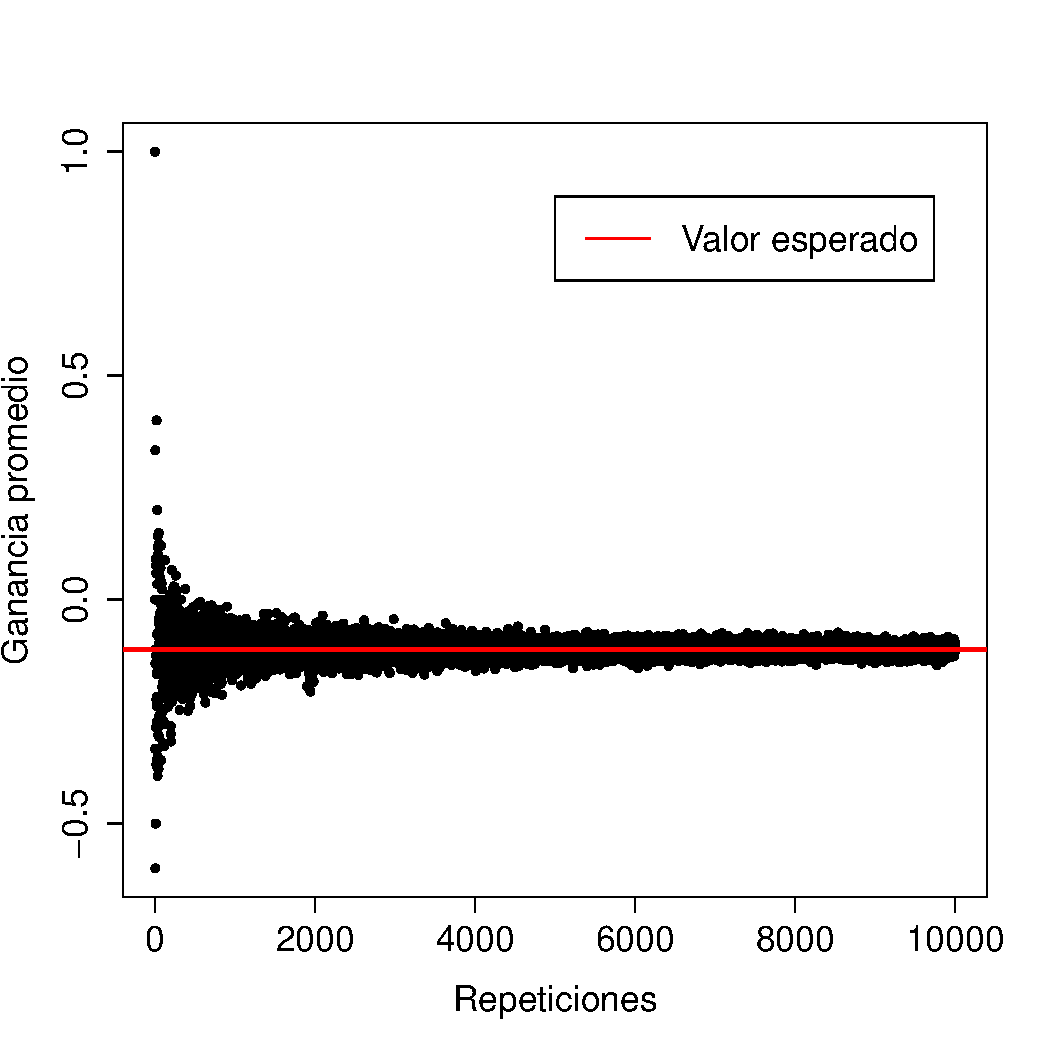
\includegraphics[width=1\textwidth]{247_1.pdf}
    \caption{P. 274, 1.}
    \label{247_1}
\end{figure}

\section*{P. 247, 6}
\emph{A die is rolled twice. Let $X$ denote the sum of the two numbers that turn up, and Y the difference of the numbers (specifically, the number on the first roll minus the number on the second). Show that $E(X Y) = E(X)E(Y )$. Are $X$ and $Y$ independent?}

Se generan $100\ 000$ tiradas de dos dados $d_1$ y $d_2$, las que se suman en $X$, se restan $Y = d_1 - d_2$ y se obtiene $XY$. Una muestra de estos resultados se halla en la tabla \ref{247_6} (p. \pageref{247_6}). 

% latex table generated in R 4.0.2 by xtable 1.8-4 package
% Mon Nov 09 16:18:28 2020
\begin{table}
    \centering
    \caption{Muestra de resultados de p. 247, 6.}
    \label{247_6}
    \begin{tabular}{cccccc}
      \hline
        $d_1$ & $d_2$ & $X$ & $Y$ & $XY$ \\ 
      \hline
        4 &   4 &   8 &   0 &   0 \\ 
        3 &   6 &   9 &  -3 & -27 \\ 
        2 &   1 &   3 &   1 &   3 \\ 
        4 &   1 &   5 &   3 &  15 \\ 
        5 &   1 &   6 &   4 &  24 \\ 
       \hline
    \end{tabular}
\end{table}

Además, se muestran los histogramas de los valores de $X$, $Y$ así como $XY$ en la figura \ref{247_6_Fig} (p. \pageref{247_6_Fig}), donde se puede constatar que los valores esperados son $E(X) = 7$, $E(Y) = 0$, $E(XY) = 0$ y $E(X) \cdot E(Y) = 0 = E(XY)$.

\begin{figure}
    \begin{subfigure}{.5\textwidth}
        \centering
        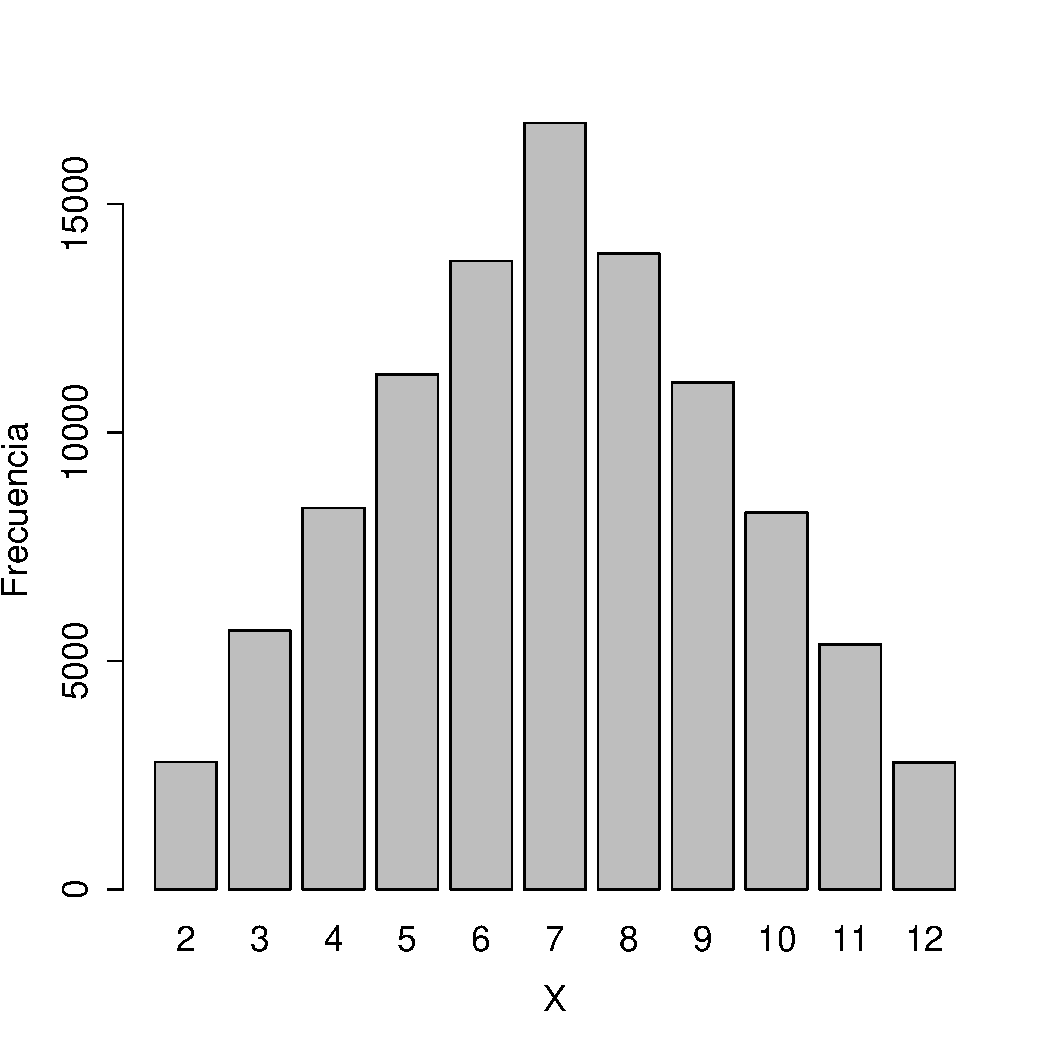
\includegraphics[scale=0.4]{247_6_X.pdf}
        \label{247_6_X}
    \end{subfigure}
    \begin{subfigure}{0.5\textwidth}
        \centering
        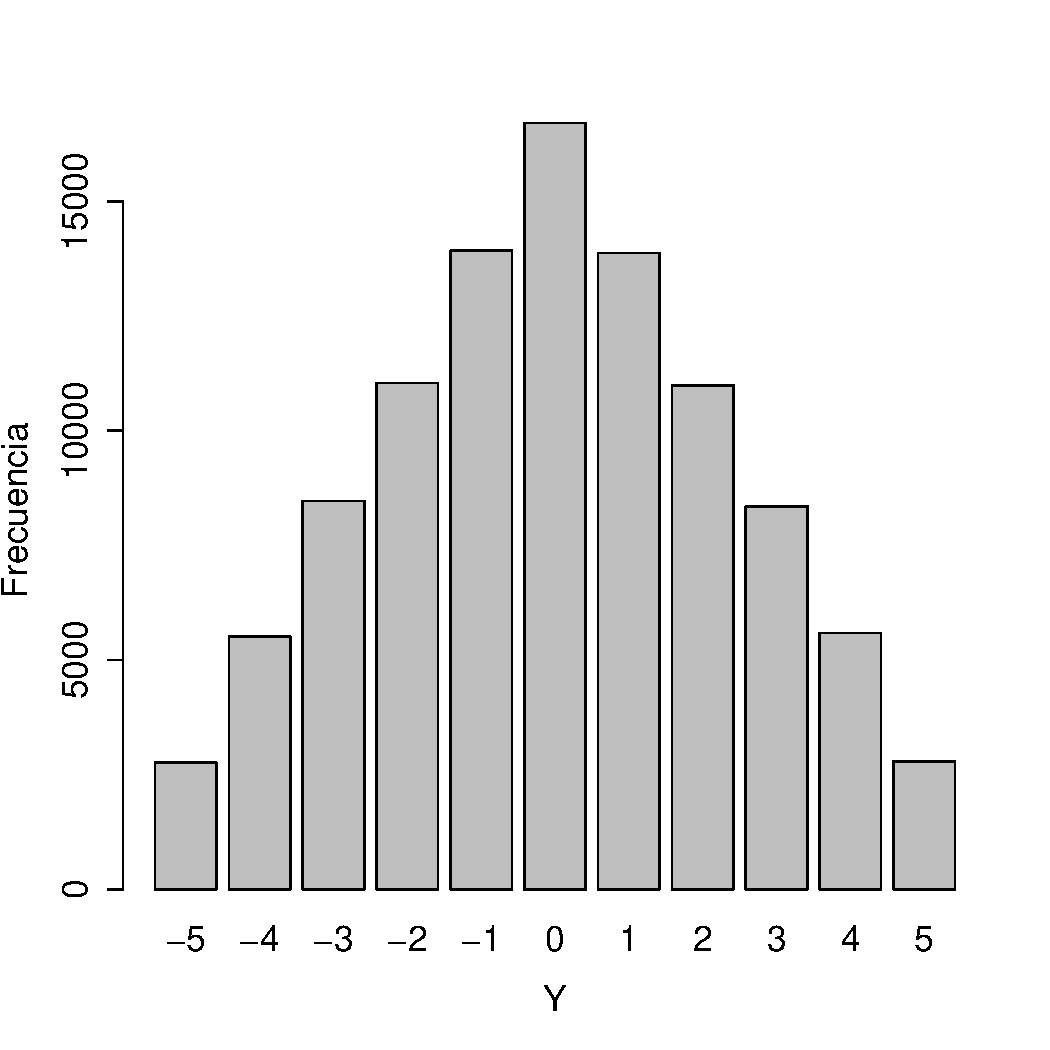
\includegraphics[scale=0.4]{247_6_Y.pdf}
        \label{247_6_Y}
    \end{subfigure}
    \begin{subfigure}{1\textwidth}
        \centering
        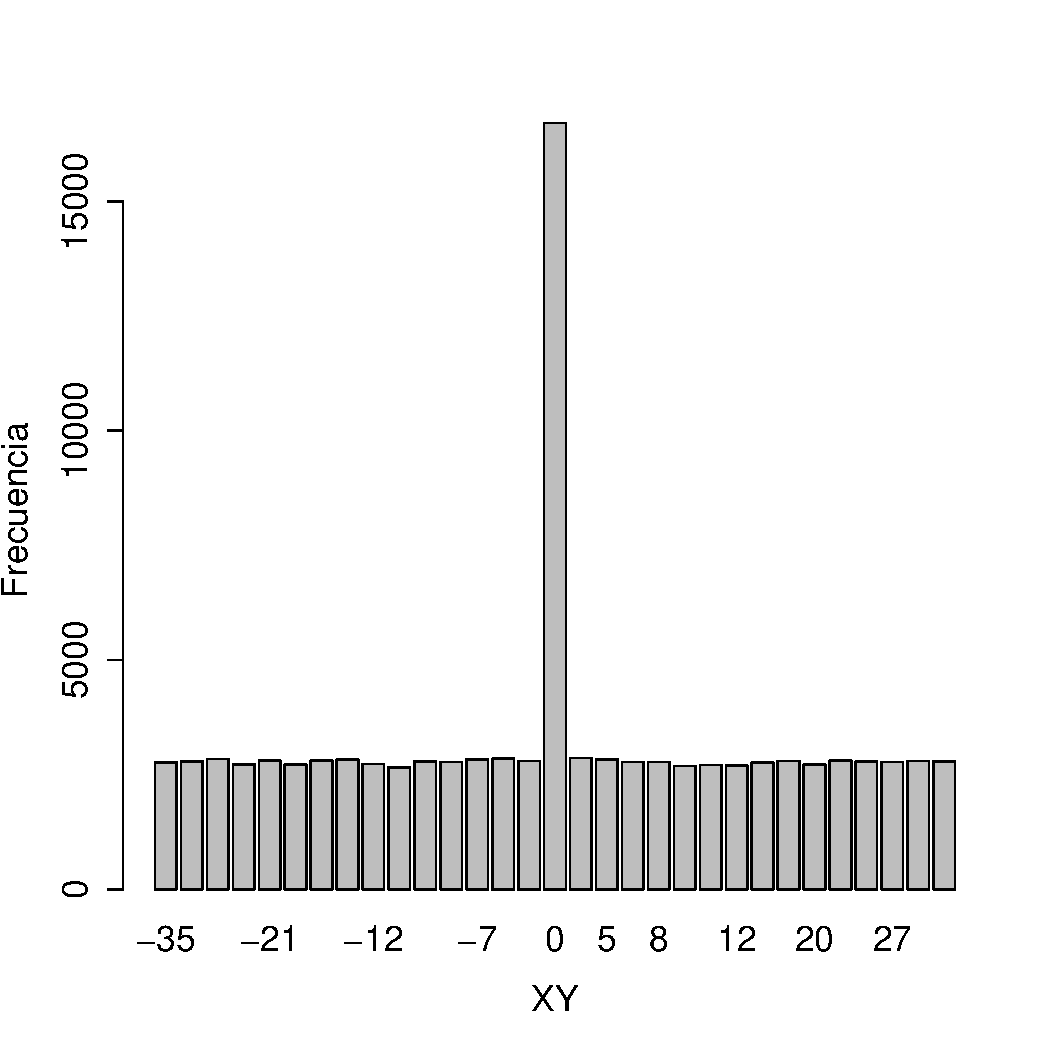
\includegraphics[scale=0.4]{247_6_XY.pdf}
        \label{247_6_XY}
    \end{subfigure}
    \caption{Histogramas de p. 247, 6.}
    \label{247_6_Fig}
\end{figure}

\section*{P. 249, 15}
\emph{A box contains two gold balls and three silver balls. You are allowed to choose successively balls from the box at random. You win 1 dollar each time you draw a gold ball and lose 1 dollar each time you draw a silver ball. After a draw, the ball is not replaced. Show that, if you draw until you are ahead by 1 dollar or until there are no more gold balls, this is a favorable game.}

En este caso, se realiza un diseño de experimentos en el que se obtienen cincuenta promedios de $10\ 000$ repeticiones del experimento mostrado en el código \ref{249_15} entre las líneas 6 a la 24. En la línea 1 se crea la variable \texttt{caja} que contiene un vector $[-1, -1, -1, 1, 1]$ análogo a los dólares que se obtienen por extraer una bola plateada, $-1$, y dorada $1$. Esta \texttt{caja} se desordena en la línea 7 y se simula la extracción una en una de las bolas en la línea 10. La variable \texttt{ganancias} declarada en la línea 3 se utiliza para almacenar las ganancias (calculadas en la línea 11) del experimento descrito, de modo que cuando se va ganando por un dólar (línea 12) o cuando han salido las dos bolas de oro (línea 16), se termina el juego y se almacenan las ganancias en la línea 22.

\begin{lstlisting}[caption={P. 249, 15}, captionpos=t, label=249_15]
caja = c(rep(-1, 3), rep(1, 2))
orden = c()
ganancias = c()
promedios = c()
for (k in 1:50){
  for (i in 1:10000){
    muestra = sample(caja)
    ganancia = 0
    oro = 0
    for (j in 1:length(caja)){
      ganancia = ganancia + muestra[j]
      if (ganancia == 1){
        break
      } else if (muestra[j] == 1){
        oro = oro + 1
        if (oro == 2){
          break
        }
      }
    }
    orden = c(orden, toString(caja))
    ganancias = c(ganancias, ganancia)
  }
  promedios = c(promedios, mean(ganancias))
}
\end{lstlisting}

La variable \texttt{orden} almacena el acomodo en que se desordenan al azar las cajas de bolas. Cinco muestras de estas combinaciones y sus ganancias dadas las reglas pueden verse en la tabla \ref{tabla:249_15} (p. \pageref{tabla:249_15}). Adicionalmente, se muestra un diagrama de cajas y bigotes con los resultados en la figura \ref{fig:249_15} (p. \pageref{fig:249_15}).

\begin{table}
    \centering
    \caption{Muestra de resultados de p. 249, 15.}
    \label{tabla:249_15}
    \begin{tabular}{lc}
      \hline
        Orden & Ganancias (USD) \\ 
      \hline
        -1, -1, -1, 1, 1 & 1 \\ 
        -1, -1, -1, 1, 1 & -1 \\ 
        -1, -1, -1, 1, 1 & 1 \\ 
        -1, -1, -1, 1, 1 & 1 \\ 
        -1, -1, -1, 1, 1 & 1 \\ 
       \hline
    \end{tabular}
\end{table}

\begin{figure}
    \centering
    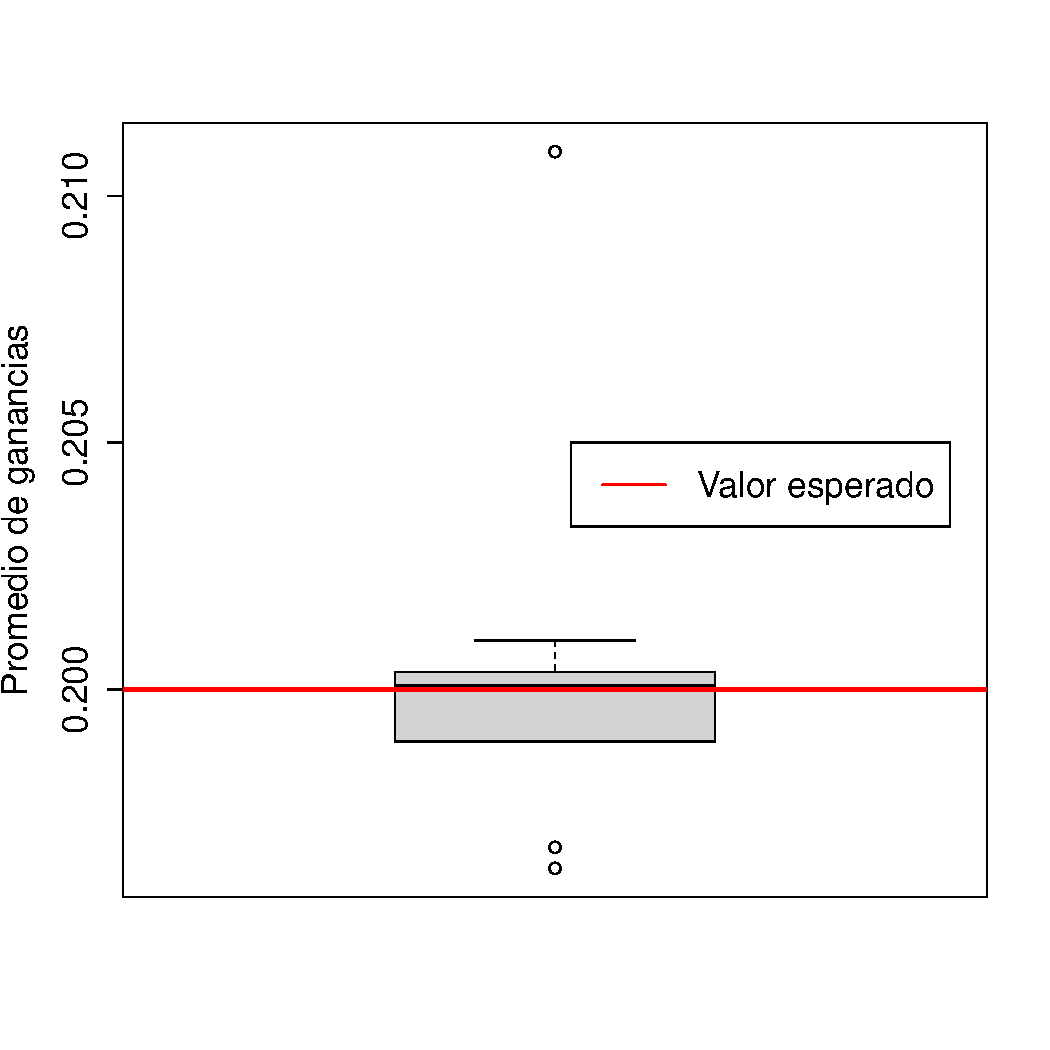
\includegraphics[width=1\textwidth]{249_15.pdf}
    \caption{Diagrama de cajas y bigotes de $50$ promedios de $10\ 000$ repeticiones para el problema P. 279, 15.}
    \label{fig:249_15}
\end{figure}

\section*{P. 249, 18}
\emph{Exactly one of six similar keys opens a certain door. If you try the keys, one after another, what is the expected number of keys that you will have to try before success?}

Se generan $100\ 000$ números aleatorios entre $0$ y $5$ que corresponden a los intentos que se harían antes de abrir la puerta mediante \texttt{sample(0:5, 100000, replace = TRUE)}. La media de esos intentos es aproximadamente $2.5$.

\section*{P. 249, 19}
\emph{A multiple choice exam is given. A problem has four possible answers, and exactly one answer is correct. The student is allowed to choose a subset of the four possible answers as his answer. If his chosen subset contains the correct answer, the student receives three points, but he loses one point for each wrong answer in his chosen subset. Show that if he just guesses a subset uniformly and randomly his expected score is zero.}

Esto se puede lograr a partir del procedimiento mostrado en el código \ref{249_19}, mediante el cálculo de la media (línea 1) de $100\ 000$ repeticiones (línea 3) de la suma (línea 4) de los valores de respuestas (línea 6) de un subconjunto elegido al azar de esas respuestas (línea 7). La función \texttt{unlist} permite convertir la lista resultante de la función \texttt{lapply} en un vector al que se le puede aplicar la función \texttt{mean}.

\begin{lstlisting}[caption={P. 249, 19}, captionpos=t, label=249_19]
mean(
  unlist(
    lapply(1:100000, 
      function(x) {
        sum(
          sample(c(-1, -1, -1, 3), 
            sample(1:4)
          )
        )
      }
    )
  )
)
\end{lstlisting}

\section*{P. 263, 1}
\emph{A number is chosen at random from the set \( S = \lbrace -1, 0, 1 \rbrace \). Let \(X\) be the number chosen. Find the expected value, variance, and standard deviation of \(X\).}

Es posible usar las funciones \texttt{mean}, \texttt{var} y \texttt{sd} de R a una muestra de un millón de valores del arreglo $S = \lbrace -1, 0, 1 \rbrace$, dado por la instrucción \texttt{sample(c(-1, 0, 1), 1000000, replace=TRUE)}. Estos valores son $E^*(X) = -0.0007 \approx E(X) = 0$; $V^*(X) = 0.6669 \approx V(X) = 2/3$; y $D^*(X) = 0.8164 \approx D(X) = \sqrt{2/3}$.

\section*{P. 264, 9}
\emph{A die is loaded so that the probability of a face coming up is proportional to the number on that face. The die is rolled with outcome $X$. Find $V(X)$ and $D(X)$.}

La función \texttt{sample} de R permite asignar probabilidades a los elementos de un vector sobre el que se desean extraer muestras con el uso del atributo \texttt{prob}, de modo que \texttt{sample(1:6, prob = (1/21 * 1:6), 100000, replace = T)} devuelve $100\ 000$ valores entre $[1, 2, 3, 4, 5, 6]$ con probabilidades $[\frac{1}{21}, \frac{2}{21}, \frac{3}{21}, \frac{4}{21}, \frac{5}{21}, \frac{6}{21}]$ respectivamente, a los cuales se les puede calcular el promedio, varianza y desviación estándar con \texttt{mean}, \texttt{var} y \texttt{sd}. Los resultados, en ese orden, son $4.3388$, $2.2129$, $1.4876$, muy cercanos a los calculados analíticamente.


\section*{P. 278, 3}
\emph{The lifetime, measure in hours, of the ACME super light bulb is a random variable T with density function \(f_T (t) = \lambda^2 te^{- \lambda t}\), where \(\lambda = 0.05\). What is the expected lifetime of this light bulb? What is its variance?}

La probabilidad de una variable aleatoria continua $x$ en un intervalo $[a, b]$ se calcula mediante
\begin{dmath*}
    P(a \leq x \leq b) = \int_a^b f_x(X) \mathrm{d}X,
\end{dmath*}
mientras que su valor esperado es
\begin{dmath*}
    E(X) = \int x f_X(x) \mathrm{d}x
\end{dmath*}
y la varianza
\begin{dmath*}
    \text{Var}(X) = \int (x - \mu_X)^2 f_X(x) \mathrm{d}x.
\end{dmath*}

En este problema,  
\begin{dmath}
    \label{eq1}
    f_T (t) = 0.05^2 te^{- 0.05 t}.
\end{dmath}

Esto se puede calcular en R con el uso de la función \texttt{integrate}, lo cual se realiza en el código \ref{278_3}, donde se definen \texttt{f} como $f_T(t)$, \texttt{g} como $E(T)$ y \texttt{h} como $V(T)$. Posteriormente se usa \texttt{integrate} para calcular las integrales de las variables \texttt{g} y \texttt{h}.

\begin{lstlisting}[caption={P. 278, 3; solución analítica}, captionpos=t, label=278_3]
f <- function(t) 0.05^2 * t * exp(-0.05 * t)
g <- function(t) t * f(t)
h <- function(t) t^2 * f(t)

E <- integrate(g, lower = 0, upper = Inf)$value
V <- integrate(h, lower = 0, upper = Inf)$value
\end{lstlisting}

Como la ecuación \ref{eq1} es una función de distribución, se pueden calcular las probabilidades de valores aleatorios. Así, para este caso, se generan un millón de valores aleatorios entre $0$ y $100$ con \texttt{a = runif(100000, 0, 150)} y luego sus probabilidades con \texttt{p = f(a)}. Un histograma de la función de distribución de esta variable se encuentra en la figura \ref{278_3} (p. \pageref{278_3}). Posteriormente, se obtienen un millón de valores aleatorios del vector \texttt{a} con las probabilidades almacenadas en el vector \texttt{p} mediante la variable \texttt{s} donde se almacena \texttt{sample(a, 100000, prob=p, replace=TRUE)}, con lo que se puede calcular tanto el valor esperado como el promedio de esos valores, obtenido por la función \texttt{mean}, y la varianza con \texttt{var}, como se observa en el código \ref{278_3_b}

\begin{lstlisting}[caption={P. 278, 3; aproximación experimental }, captionpos=t, label=278_3_b]
a = runif(100000, 0, 1000)
p = f(a)
s = sample(a, 100000, prob=p, replace=TRUE)
mean(s)
var(s)
\end{lstlisting}

\begin{figure}
    \centering
    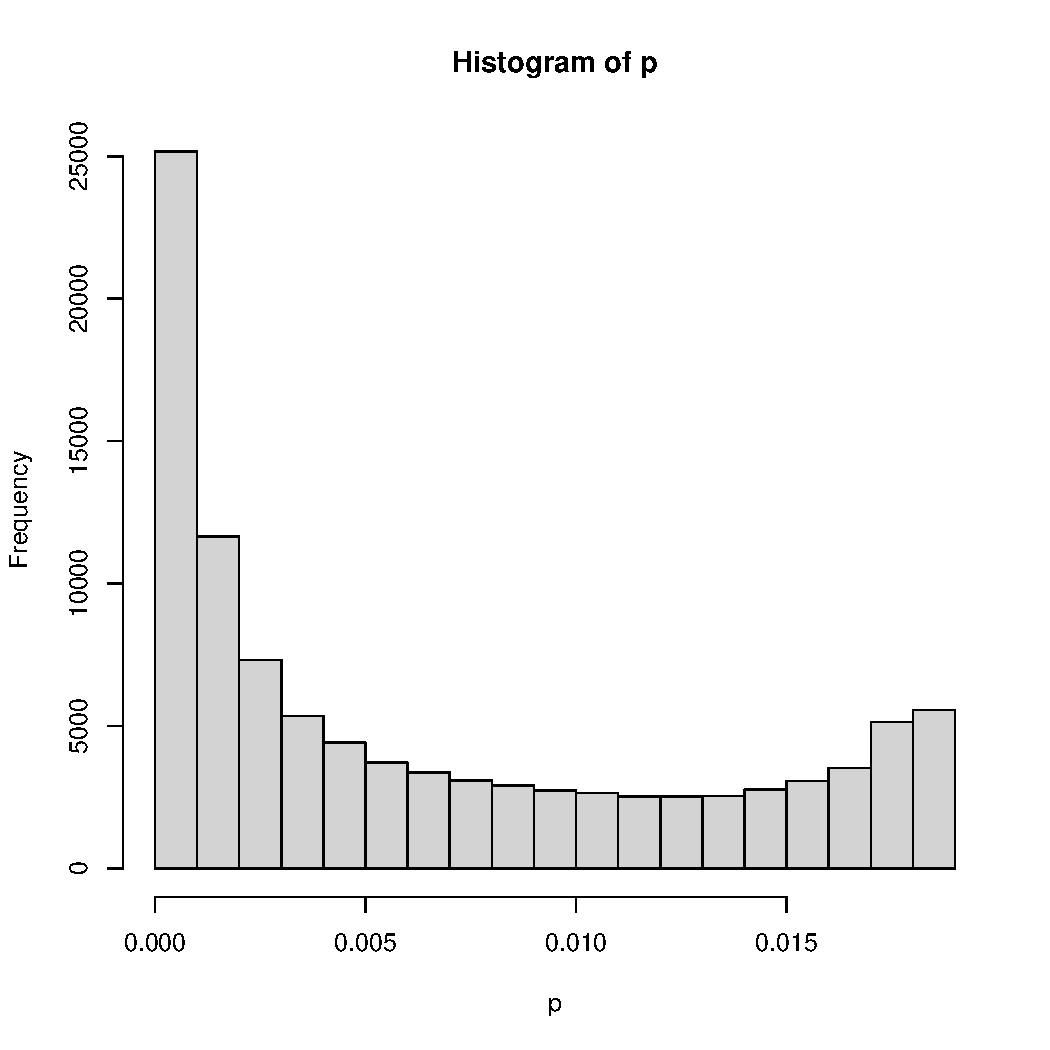
\includegraphics[width=1\textwidth]{278_3.pdf}
    \caption{Histograma de la función de distribución de probabilidades dada por la ecuación \ref{eq1} para un millón de variables aleatorias con distribución $\mathcal{U}(0, 150)$.}
    \label{fig:278_3}
\end{figure}

\end{document}